\chapter{Gaze Preserving Face Redaction}

Redaction refers is the process of hiding some sensitive information present in an image in order to preserve the privacy of individuals. The sensitive information can be present in the foreground or the background of the image. In this work, we are particularly interested in face redaction, where we hide all the faces present in an image frame by blurring or blackening out the face. As we discussed earlier, face redaction can be achieved in several modalities, e.g., the eyes can either be hidden (blurred or blacked out) or visible such that it doesn't compromise the identity of the subject. In this work, we systematically explore a feature preserving mechanism for face redaction, with our focus being on the gaze and proximity features of the face. In the next sections, we discuss our approach to gaze preservation.


%%%%%%%%%%
\section{Our Prior Work on Gaze Classification}
Our prior work on gaze classification aimed to build a 3-way gaze classifier on the 3-way UK dataset. In order to do so, we utilized the concept of Transfer Learning, which consists of 2 phases of training. In the 1st training phase, a regression model is trained on the entire MIT dataset. We used the Dlib HOG extractor to extract the face and eyes. This regression model is called the pre-trained base regression model since transfer learning is applied over this already trained model. Note that this pre-trained model has been trained for a different task (i.e., regression) on a different dataset (i.e., MIT dataset) than our requirement.

Now, this model is modified as follows as depicted in figure \ref{fig:TransferLearning}:
\begin{enumerate}
  \item Add a neuron at the final layer (so that the final layer has 3 output neurons) to output L, R, C.
  \item Freeze the weights of initial layers (also called fixed layers) and leave the remaining layers as trainable. This means that during the 2nd training phase, the weights of fixed layers will not be updated and will remain fixed.
  \item Replace MSE Loss with Cross-Entropy Loss.
  \item Train a 3-Way Classifier on UK dataset with the above-modified model, which is the 2nd phase of training (also referred to as the tuning phase).
\end{enumerate}

\begin{figure}[h]
  \centering
    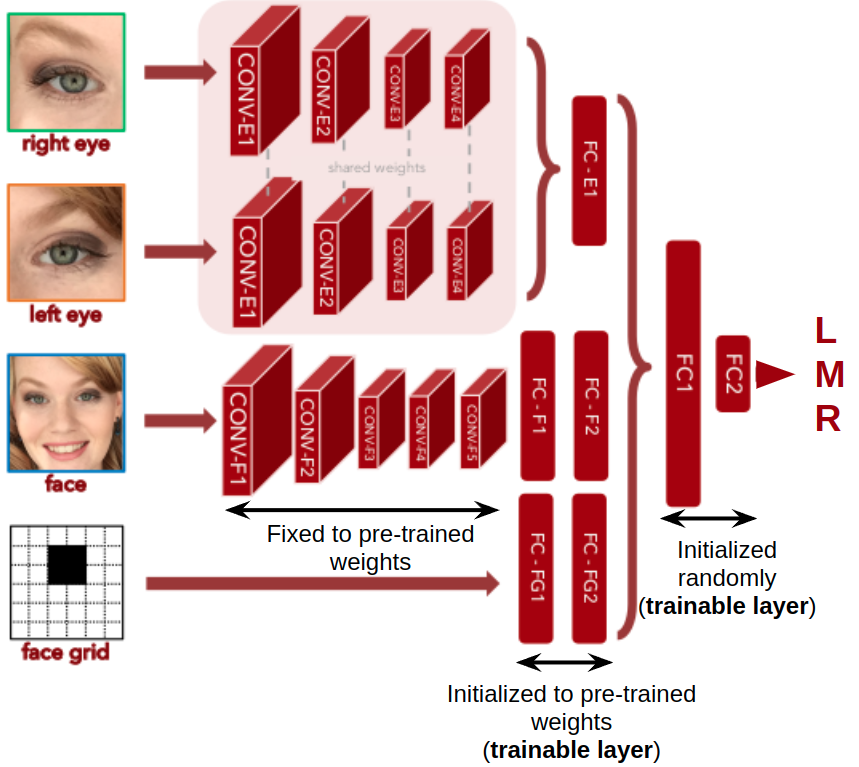
\includegraphics[scale=0.4]{GazePreservingRedaction/TransferLearning}
    \caption{Transfer Learning for 3-Way Gaze Classification}
    \label{fig:TransferLearning}
\end{figure}

By using the above approach, we got an accuracy (the percentage of frames in which the network predicted the correct gaze class labels) of 88.65\% on the 3-way UK dataset. For our current work on feature preserving gaze classification, we use the same base regression model in the tuning approaches (discussed in the following sections), which we trained on MIT data for the transfer learning approach.


%%%%%%%%%%
\section{3-Way Gaze Classification on UK data}
We first train a base regression model on the MIT dataset, which outputs XY gaze coordinates. Then we tune the model for 3-way gaze classification on 3-way UK data according to the schemes discussed in the following sub-sections.


%%%
\subsection{Tuning with Redacted Faces}
Our aim is to perform gaze classification by taking redacted faces as inputs. In this direction, we first tune the base regression model and test with various redaction schemes. We tuned the model for 10 epochs on around 0.4 million images in the train set and tested our model on 0.1 million images. We used the Cross-entropy loss function for training with stochastic gradient descent algorithm.

\begin{table}[h]
  \centering
    \caption{Accuracy of 3-way classifier tuned with redacted faces}
    \label{tab:3way_tune-redactedFaces}
    \begin{tabular}{ | >{\centering\arraybackslash} m{2.55cm} || >{\centering\arraybackslash} m{1.6cm} | >{\centering\arraybackslash} m{1.3cm} | >{\centering\arraybackslash} m{1.3cm} | >{\centering\arraybackslash} m{1.3cm} | >{\centering\arraybackslash} m{1.3cm} | >{\centering\arraybackslash} m{2.2cm} |}
        \hline
         & 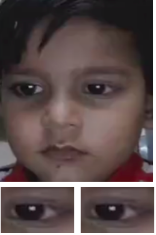
\includegraphics[scale=0.2,valign=m]{GazePreservingRedaction/No_redaction} & 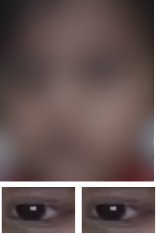
\includegraphics[scale=0.2,valign=m]{GazePreservingRedaction/Face_blurred} & 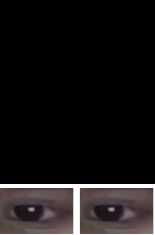
\includegraphics[scale=0.2,valign=m]{GazePreservingRedaction/Face_blacked} & 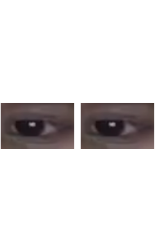
\includegraphics[scale=0.2,valign=m]{GazePreservingRedaction/No_face} & 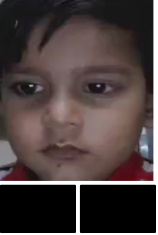
\includegraphics[scale=0.2,valign=m]{GazePreservingRedaction/Eyes_blacked} & 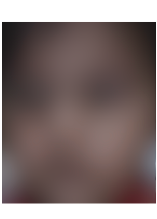
\includegraphics[scale=0.2,valign=m]{GazePreservingRedaction/Face_blurred_No_eyes} \\
        \hline
        \textbf{Scheme} & No redaction & Face blurred & Face blacked & No face & Eyes blacked & Face blurred + No eyes \\
        \hline
        \textbf{Accuracy (\%)} & 83.42 & 82.60 & 82.56 & 82.74 & 52.62 & 39.26 \\
        \hline
    \end{tabular}
\end{table}
% \todo{See if table header can be made in 2 lines via above code}

% \begin{table}[h]
%   \centering
%     \caption{Accuracy of 3-way classifier tuned with redacted faces}
%     \label{tab:3way_tune-redactedFaces}
%     \begin{tabularx}{1.0\textwidth}{| >{\centering\arraybackslash}X || >{\centering\arraybackslash}X | >{\centering\arraybackslash}X | >{\centering\arraybackslash}X | >{\centering\arraybackslash}X | >{\centering\arraybackslash}X | >{\centering\arraybackslash}X |}
%       \hline
%       \textbf{Scheme} & No redaction & Face blurred & Face blacked out & No face & Eyes blacked out & Face blurred + No eyes \\
%       \hline
%       \textbf{Accuracy (\%)} & 83.42 & 82.60 & 82.56 & 82.74 & 52.62 & 39.26 \\
%       \hline
%     \end{tabularx}
% \end{table}

As can be seen in table \ref{tab:3way_tune-redactedFaces}, the accuracy of approximately 82\% demonstrates that our approach to face redaction preserves the 3-way gaze classes. The good accuracy with "No face" denotes the accuracy of the model when no face input was provided to the model, but note that, as shown in the table, the eye crops are provided to the model. So, the model is able to learn to predict gaze based solely on the presence of eyes. The last two columns also show that the model is able to learn to emphasize on eyes for gaze classification.


%%%
\subsection{Tuning with Visible Faces}
In the previous section, we tuned the model on redacted faces to obtain gaze classification accuracies around 82 \%. It would be interesting to see the accuracy results if the model is tuned on visible faces and tested on redacted faces. In this direction, we tune the base regression model with faces visible in the image frame (i.e., no redaction) and test the tuned model with various redaction schemes. It would be useful if we could get a high accuracy model for gaze classification with redacted faces just by training (i.e., tuning) the base model with unredacted faces.

\begin{table}[h]
  \centering
    \caption{Accuracy of 3-way classifier tuned with visible faces}
    \label{tab:3way_tune-visibleFaces}
    \begin{tabular}{|c||c|c|c|c|}
      \hline
         & 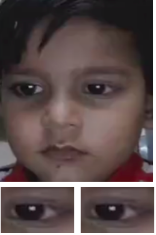
\includegraphics[scale=0.2,valign=m]{GazePreservingRedaction/No_redaction} & 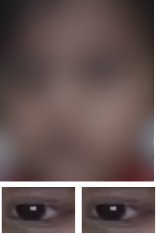
\includegraphics[scale=0.2,valign=m]{GazePreservingRedaction/Face_blurred} & 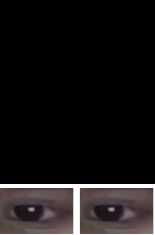
\includegraphics[scale=0.2,valign=m]{GazePreservingRedaction/Face_blacked} & 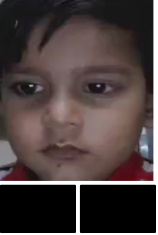
\includegraphics[scale=0.2,valign=m]{GazePreservingRedaction/Eyes_blacked} \\
      \hline
      \textbf{Scheme} & No redaction & Face blurred & Face blacked out & Eyes blacked out \\
      \hline
      \textbf{Accuracy (\%)} & 88.65 & 86.86 & 86.63 & 39.98 \\
      \hline
    \end{tabular}  
\end{table}

We can see from table \ref{tab:3way_tune-visibleFaces} that testing with redacted (blurred or blacked out) faces results in accuracy almost equal to the baseline result when testing with no redaction. This shows that training (i.e., tuning) with redacted faces is not necessary to obtain a high-performance model for redacted faces. It is also evident from the result obtained with testing on redacted eyes that the model is able to differentiate and emphasize on the eyes for classifying gaze accurately.


%%%%%%%%%%
\section{2-Way Gaze Classification on UK data}
Similar to the 3-way gaze classification performed on the 3-way UK dataset, we test the performance of our feature preserving face redaction approach for 2-way gaze classification on the filtered 2-way UK dataset. The same base regression model (i.e., regression model trained on MIT data) is used for the experiments in the following subsections.


%%%
\subsection{Post-classification}
Since the base regression model outputs XY gaze coordinates, it is relatively easier to perform a post-classification of the coordinates into gaze classes according to the device screen dimensions and camera location. This method is the most straightforward way for classification, given a regression model.

\begin{table}[h]
  \centering
    \caption{Accuracy of post-classification on filtered 2-way UK data}
    \label{tab:2way_postClassif_UK}
    \begin{tabular}{|c||c|c|c|c|}
      \hline
         & 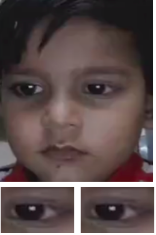
\includegraphics[scale=0.2,valign=m]{GazePreservingRedaction/No_redaction} & 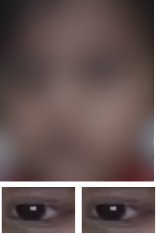
\includegraphics[scale=0.2,valign=m]{GazePreservingRedaction/Face_blurred} & 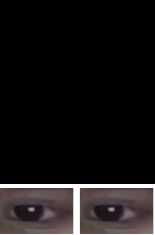
\includegraphics[scale=0.2,valign=m]{GazePreservingRedaction/Face_blacked} & 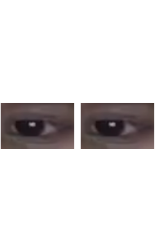
\includegraphics[scale=0.2,valign=m]{GazePreservingRedaction/No_face} \\
      \hline
      \textbf{Scheme} & No redaction & Face blurred & Face blacked out & No face \\
      \hline
      \textbf{Accuracy (\%)} & 64.35 & 54.63 & 53.63 & 53.71 \\
      \hline
    \end{tabular}  
\end{table}

Table \ref{tab:2way_postClassif_UK} shows that the method of post-classification does not work accurately for classification, and the regression model under-performs on the classification task. A possible explanation for this is the non-generalizability of the regression model due to domain shift in data distribution (note that the regression model is trained on MIT data collected on iPhones/iPads, whereas testing is done on UK data collected on UK device).


%%%
\subsection{Tuning with Redacted Faces}
As demonstrated in table \ref{tab:2way_postClassif_UK}, the post-classification model doesn't generalize well due to data domain shift in data distribution. So, we need to tune the regression model on the filtered 2-way UK data to adapt to the data distribution shift between the data on which the regression model is trained and data on which 2-Way classification is targeted. Note that we train (i.e., tune) the model on a subset of filtered 2-way UK data (2.5\% of the "train" set) due to the enormous dataset size. This helps to make the training faster as well as check if the model is able to fit properly with a small amount of data.

\begin{table}[h]
  \centering
    \caption{Accuracy of 3-way classifier tuned with redacted faces}
    \label{tab:2way_tune-UK}
    \begin{tabular}{ | >{\centering\arraybackslash} m{2.55cm} || >{\centering\arraybackslash} m{1.6cm} | >{\centering\arraybackslash} m{1.2cm} | >{\centering\arraybackslash} m{1.3cm} | >{\centering\arraybackslash} m{0.9cm} | >{\centering\arraybackslash} m{1.3cm} | >{\centering\arraybackslash} m{2.2cm} | >{\centering\arraybackslash} m{1.3cm} |} 
        \hline
         & 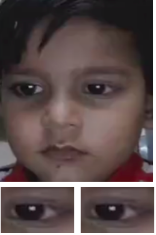
\includegraphics[scale=0.2,valign=m]{GazePreservingRedaction/No_redaction} & 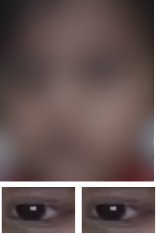
\includegraphics[scale=0.2,valign=m]{GazePreservingRedaction/Face_blurred} & 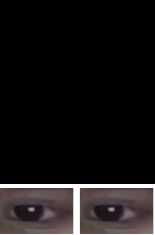
\includegraphics[scale=0.2,valign=m]{GazePreservingRedaction/Face_blacked} & 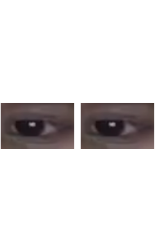
\includegraphics[scale=0.2,valign=m]{GazePreservingRedaction/No_face} & 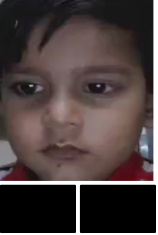
\includegraphics[scale=0.2,valign=m]{GazePreservingRedaction/Eyes_blacked} & 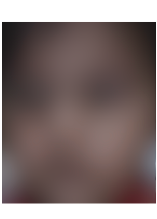
\includegraphics[scale=0.2,valign=m]{GazePreservingRedaction/Face_blurred_No_eyes} &
         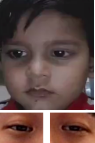
\includegraphics[scale=0.32,valign=m]{GazePreservingRedaction/Dummy_eyes} \\
        \hline
        \textbf{Scheme} & No redaction & Face blurred & Face blacked & No face & Eyes blacked & Face blurred + No eyes & Dummy eyes \\
        \hline
        \textbf{Accuracy (\%)} & 96.77 & 96.78 & 96.75 & 97.09 & 74.93 & 51.36 & 75.63 \\
        \hline
    \end{tabular}
\end{table}
% \todo{See if table header can be made in 2 lines via above code}

% \begin{table}[h]
%   \centering
%     \caption{Accuracy of 2-way classifier tuned on UK data}
%     \label{tab:2way_tune-UK}
%     \begin{tabularx}{1.0\textwidth}{| >{\centering\arraybackslash}X || >{\centering\arraybackslash}X | >{\centering\arraybackslash}X | >{\centering\arraybackslash}X | >{\centering\arraybackslash}X | >{\centering\arraybackslash}X | >{\centering\arraybackslash}X | >{\centering\arraybackslash}X}
%       \hline
%       \textbf{Scheme} & No redaction & Face blurred & Face blacked out & No face & Eyes blacked out & Face blurred + No eyes & Dummy eyes \\
%       \hline
%       \textbf{Accuracy (\%)} & 96.77 & 96.78 & 96.75 & 97.09 & 74.93 & 51.36 & 75.63 \\
%       \hline
%     \end{tabularx}
% \end{table}

The results in table \ref{tab:2way_tune-UK} show that our proposed tuning model is as accurate on redacted faces as a model on unredacted faces. We also perform ablation studies by redacting the eyes with different variations instead of the face in order to decide if we really need to provide eye crops in our face redacted dataset (i.e., to check the accuracy of possible approaches a client would use with our dataset if we don’t provide eye crops). The above results clearly demonstrate that eye crops are important for gaze classification, and the model is able to learn to focus on eye crops.


%%%
\subsection{Training Classifier from scratch}
The above approaches to feature preserving gaze classification use a regression model as the base model, where the model weights are learned using MIT data. In the absence of such a model, it is logical to train a classifier directly from scratch. We train two classifiers, one on a subset of filtered 2-way UK data (2.5\% of the "train" set) and the other on the full dataset.

\begin{table}[h]
  \centering
    \caption[Accuracy of classifier on filtered 2-way UK data]{Accuracy of classifier trained from scratch on filtered 2-way UK data}
    \label{tab:2way_directClassif_UK}
    \begin{tabular}{|c||c|c|c|c|}
      \hline
      & \multicolumn{2}{c|}{\textbf{Subset (2.5\%) UK data}} & \multicolumn{2}{c|}{\textbf{Full UK data}} \\
      \hline
      \textbf{Scheme} & No redaction & Face blurred & No redaction & Face blurred \\
      \hline
      \textbf{Accuracy (\%)} & 50.95 & 51.60 & 96.06 & 96.35 \\
      \hline
    \end{tabular}  
\end{table}

Results in table \ref{tab:2way_directClassif_UK} show that training a classifier model from scratch requires a large data for learning since, with a subset of 2.5\% data, the 2-way classifier is as good as a random classifier (with 50\% accuracy). This demonstrates the utility of our app, which can generate curated 3-Way data in abundance, from which a sophisticated 2-way dataset can be prepared. In the presence of such an app and the availability of a large dataset, we can see that the gaze classification with redaction performs equally well as without redaction.


%%%%%%%%%%
\section{2-Way Gaze Classification on START data}
The UK dataset is a curated dataset that is collected by our app dedicated to 3-way gaze classification. As such, the filtered 2-way UK data is inherently different from the 2-way dataset actually collected in the Preferential Looking task mentioned in the earlier sections. So, it is important to test our approach on the in-the-wild dataset. In this direction, we test our methods on the 2-way START dataset, which was collected in Nottingham. As noted in section 3.3, this dataset is not an in-the-wild dataset purely because although the START app was used for dataset collection, the videos were recorded in a lab environment. The following subsections demonstrate the experiments performed on this dataset for gaze preserving redaction.


%%%
\subsection{Post-Classification}
Similar to the post-classification method adopted earlier, we perform a post-classification procedure on the output of the base regression model. Note that, unlike the UK device, the START device has its camera at an offset of 2 cm towards the left of the center of the long edge of the device. So, the demarcation for left and right gaze labels for this device does not go through the camera.

\begin{table}[h]
  \centering
    \caption{Accuracy of post-classification on 2-way START data}
    \label{tab:2way_postClassif_START}
    \begin{tabular}{|c||c|c|c|c|}
      \hline
         & 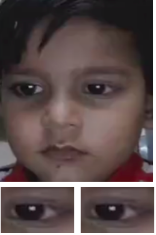
\includegraphics[scale=0.2,valign=m]{GazePreservingRedaction/No_redaction} & 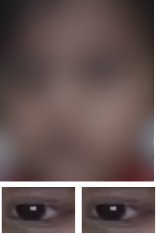
\includegraphics[scale=0.2,valign=m]{GazePreservingRedaction/Face_blurred} & 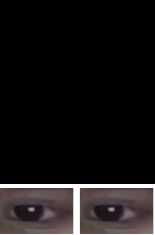
\includegraphics[scale=0.2,valign=m]{GazePreservingRedaction/Face_blacked} & 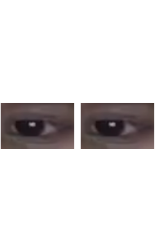
\includegraphics[scale=0.2,valign=m]{GazePreservingRedaction/No_face} \\
      \hline
      \textbf{Scheme} & No redaction & Face blurred & Face blacked out & No face \\
      \hline
      \textbf{Accuracy (\%)} & 65.11 & 52.93 & 49.53 & 63.15 \\
      \hline
    \end{tabular}  
\end{table}

The results shown above in table \ref{tab:2way_postClassif_START} for post-classification show consistent results as in table \ref{tab:2way_postClassif_UK}. This further strengthens our argument that the method of post-classification does not work accurately for classification, and the regression model underperforms on the classification task due to the non-generalizability of the regression model arising because of the domain shift in data distribution.


%%%
\subsection{Tuning with Redacted Faces}
As demonstrated in table \ref{tab:2way_postClassif_START}, the post-classification model doesn't generalize well due to data domain shift in data distribution. So, we need to tune the regression model on the 2-way START data to adapt to the data distribution shift between the data on which the regression model is trained and data on which 2-Way classification is targeted. Note that we train (i.e., tune) the model on a subset of 2-way START data (i.e., 10\% of the "train" set) to check the effectiveness of tuning the model with a small amount of data. This helps to make the training faster, check if the model is able to fit properly with a small amount of data, and make a fair comparison with the tuning results on filtered 2-way UK data presented in section 2.2 of this chapter.

\begin{table}[h]
  \centering
    \caption{Accuracy of 2-way classifier tuned on START data}
    \label{tab:2way_tune-START}
    \begin{tabular}{|c||c|c|c|c|}
      \hline
         & 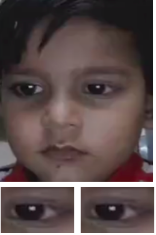
\includegraphics[scale=0.2,valign=m]{GazePreservingRedaction/No_redaction} & 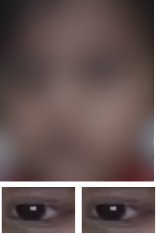
\includegraphics[scale=0.2,valign=m]{GazePreservingRedaction/Face_blurred} & 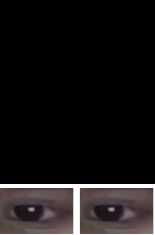
\includegraphics[scale=0.2,valign=m]{GazePreservingRedaction/Face_blacked} & 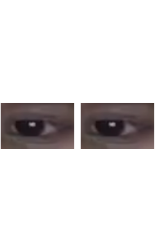
\includegraphics[scale=0.2,valign=m]{GazePreservingRedaction/No_face} \\
      \hline
      \textbf{Scheme} & No redaction & Face blurred & Face blacked out & No face \\
      \hline
      \textbf{Accuracy (\%)} & 93.94 & 94.07 & 93.94 & 91.8 \\
      \hline
    \end{tabular}  
\end{table}

As compared to tuning results on filtered 2-way UK data (table \ref{tab:2way_tune-UK}), the tuning results on 2-way START data (table \ref{tab:2way_tune-START}) are approximately 2-3\% lower since the START dataset is a difficult dataset as compared to the well-curated filtered 2-way UK data. But the high accuracy results show that our gaze preserving face redaction approach works well on START data as well.


%%%
\subsection{Tuning with Redacted Faces on UK data and testing on START data}

\begin{figure}[h]
    \centering
    \captionsetup[subfigure]{justification=centering}
    \subfloat[2-Way START device screen]{{
        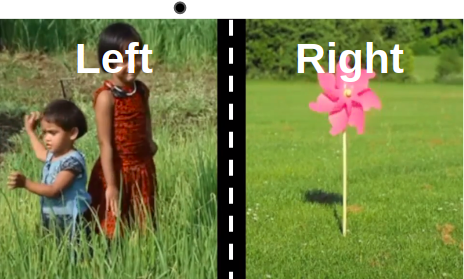
\includegraphics[width=0.3\textwidth,valign=m]{GazePreservingRedaction/2Way_vs_3Way-1}
        }}
    \quad
    \subfloat[3-Way UK device screen]{{
        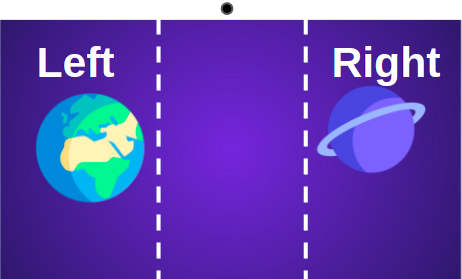
\includegraphics[scale=0.3,valign=m]{GazePreservingRedaction/2Way_vs_3Way-2}
    }}
    \caption{Contrast between 2-Way and 3-Way devices}
    \label{fig:2waySTARTdevice_vs_3wayUKdevice}
\end{figure}

Since filtered 2-way UK data is inherently different from 2-way START data, it is imperative that we test the models trained on filtered 2-way UK data on the 2-way START data in order to do justice to the 2-way premise. Figure \ref{fig:2waySTARTdevice_vs_3wayUKdevice} shows the differences between the 2-way START device and the 3-way UK device. The camera is located at an offset of 2 cm towards left from the center, as opposed to the camera located at the center of the 3-way UK device. Also, it helps in inferring the generalizability potential in the sense of the variability in the subject's age. So, we tune the base regression model on filtered 2-way UK data and directly test it on 2-way START data.

\begin{table}[h]
  \centering
    \caption{Accuracy of 2-way classifier on START data when tuned on UK data}
    \label{tab:2way_tune-UK_test-START}
    \begin{tabular}{|c||c|c|c|c|}
      \hline
         & 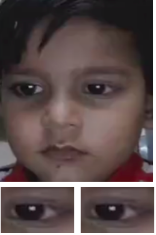
\includegraphics[scale=0.2,valign=m]{GazePreservingRedaction/No_redaction} & 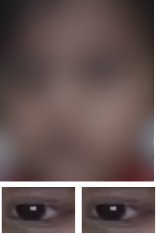
\includegraphics[scale=0.2,valign=m]{GazePreservingRedaction/Face_blurred} & 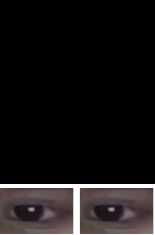
\includegraphics[scale=0.2,valign=m]{GazePreservingRedaction/Face_blacked} & 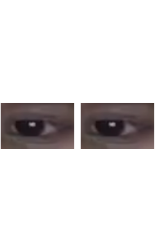
\includegraphics[scale=0.2,valign=m]{GazePreservingRedaction/No_face} \\
      \hline
      \textbf{Scheme} & No redaction & Face blurred & Face blacked out & No face \\
      \hline
      \textbf{Accuracy (\%)} & 93.12 & 93.00 & 93.00 & 93.88 \\
      \hline
    \end{tabular}  
\end{table}

The result in the above table \ref{tab:2way_tune-UK_test-START} establishes an important result that the classifier trained by tuning the model on a particular device is device-independent (given the devices are not wildly different in terms of the screen size and camera location) and generalizes well enough to yield accuracy above 93\%. This is contrary to the behavior of a regression model, which does not generalize well to other devices (as seen in sections 4.3.1 and 4.4.1 of this chapter on post-classification).


%%%%%%%%%%
\section{3-Way from 2-Way Gaze Classifier}
The 3-way gaze classification problem differs from the 2-way gaze classification problem in only the number of output gaze labels. With this insight in mind, we try to perform 3-way gaze classification from a 2-way gaze classification model. We know that in a binary classification task such as 2-way, the network predicts an output probability for left and right gaze labels, and the probability of $0.5$ inherently distinguishes the binary labels. We utilize these output probabilities to our advantage and set a window of probability $P_w$ across $0.5$ ($P_w/2$ on each side) to denote the "Middle" gaze label. Therefore, if the probability of "Left" gaze is smaller than $0.5 - P_w/2$ (making the probability of "Right" label to be greater than $0.5 + P_w/2$, since the probabilities sum to $1.0$), the output is "Right" gaze. Similarly, if the probability of "Left" gaze is greater than $0.5 + P_w/2$ (making the probability of "Right" label to be smaller than $0.5 - P_w/2$), then the output is "Left" gaze. But if the probabilities of both "Left" and "Right" gaze labels fall in the range $[0.5 - P_w/2, 0.5 + P_w/2]$, then it implies that the network is not sure whether the output is "Left" or "Right". We utilize this uncertainty of the model to predict the "Middle" gaze label as output.

We use the 2-way gaze classifier tuned on filtered 2-way UK data for carrying out the analysis above. We first obtain the 3-way gaze classification accuracies on "val" set of 3-way UK data by setting different probability windows $P_w$ for "Middle" gaze label and obtaining the probability window $P_w^{max}$ for which the accuracy is maximum. Then, we compute the 3-way accuracy on "test" set of 3-way UK data by setting the "Middle" probability window as $P_w^{max}$.

\begin{figure}[h]
    \centering
    \captionsetup[subfigure]{justification=centering}
    \subfloat[3-Way from 2-Way with No Redaction]{{
        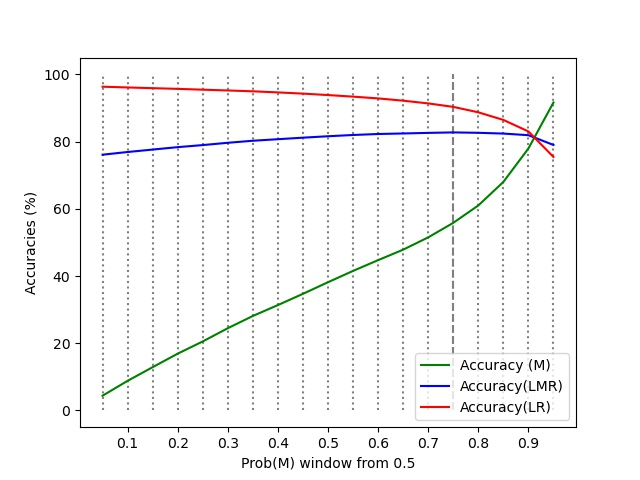
\includegraphics[scale=0.4]{GazePreservingRedaction/RF_subset2WayUK_TL_accuracy-allVal}
        \label{fig:3way_from_2way_noRedact}
        }}
    \quad
    \subfloat[3-Way from 2-Way with Redaction (Blurred Face)]{{
        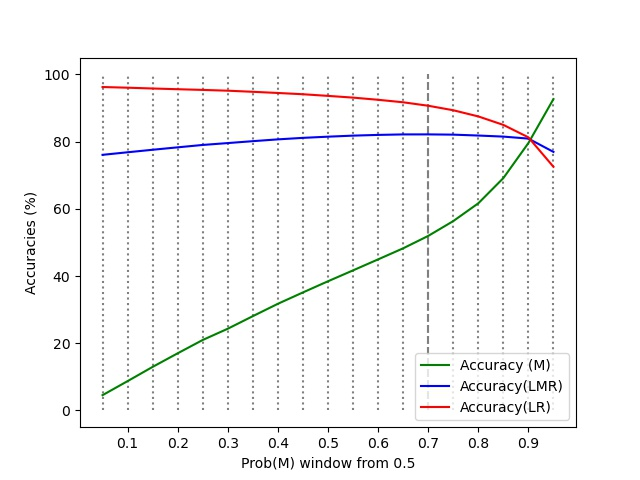
\includegraphics[scale=0.4]{GazePreservingRedaction/RF_subset2WayUK_TL-blurFace-r15_accuracy-allVal}
        \label{fig:3way_from_2way_blurFace}
    }}
    \caption[3-Way Accuracy from 2-Way model]{3-Way Accuracy from 2-Way model at various probability windows}
    \label{fig:3way_from_2way}
\end{figure}

% \begin{table}[h]
%   \centering
%     \caption{3-Way Accuracy from 2-Way model}
%     \label{tab:3way_from_2way}
%     \begin{tabular}{|c||c|c|c|}
%       \hline
%       \textbf{Scheme} & [val] Max 3-Way Accuracy & $P_w^{max}$ & [test] 3-Way Accuracy \\
%       \hline
%       \textbf{No Redaction} & 82.74 & 0.75 & 79.96 \\
%       \hline
%       \textbf{Face Blurred} & 82.14 & 0.7 & 79.83 \\
%       \hline
%     \end{tabular}  
% \end{table}

\begin{table}[h]
  \centering
    \caption{3-Way Accuracy from 2-Way model}
    \label{tab:3way_from_2way}
    \begin{tabular}{ | >{\centering\arraybackslash} m{2.55cm} || >{\centering\arraybackslash} m{2.9cm} | >{\centering\arraybackslash} m{2cm} | >{\centering\arraybackslash} m{2.2cm} |} 
        \hline
        \textbf{Scheme} & [val] Max 3-Way Accuracy & $P_w^{max}$ & [test] 3-Way Accuracy \\
        \hline
        \textbf{No Redaction} & 82.74 & 0.75 & 79.96 \\
        \hline
        \textbf{Face Blurred} & 82.14 & 0.7 & 79.83 \\
        \hline
    \end{tabular}
\end{table}

Figure \ref{fig:3way_from_2way} shows the accuracy values for the 3-way, 2-way, and for the "Middle-only" task on "val" set at varying windows of probability. Figure \ref{fig:3way_from_2way_noRedact} shows the accuracy values with no redaction and figure \ref{fig:3way_from_2way_blurFace} shows the accuracy values with redaction (i.e., blurred face). It can be seen that for both cases, the plots are very similar, thus indicating that the utilization of a 2-way gaze classification model is effective in case of redaction. As the "Middle"-only accuracy (green curve) increases rapidly on increasing the probability window, the 2-way accuracy (red curve) drops to compensate for the increasing "Middle"-only accuracy. Since we are interested in the overall 3-way accuracy, we focus on the blue curves in the plot and denote its peak with a dashed bold line. Table \ref{tab:3way_from_2way} presents the peak values of accuracy obtained on "val" set and the final "test" set accuracy obtained for the 3-way classification from the 2-way model.


\section{Extraction and Training Details}
We used Retina Face for the detection and extraction of face and eye crops for each frame in the UK and START dataset. For the extraction of 539,508 frames present in the UK dataset, Retina Face takes around 37 hours and for 7,917 frames present in the Nottingham START dataset, Retina Face takes around 30 minutes at an extraction rate of 4 frames per second.

The classification model takes a training time of around 5.3 hours per epoch on the "train" split of UK dataset, which contains 369,835 frames. In order to reduce the training time, we trained on 2.5\% subset of the UK dataset, which takes around 1.2 hours for training the model for 10 epochs.

For training the classification model, we use the Cross-entropy loss function with the Stochastic Gradient Descent (SGD) algorithm. We used a batch size of 100 for training purposes, which consumes approximately 3.5 GB memory on NVIDIA GeForce GTX 980 Ti GPU. We trained the models with a learning rate of 0.001, a momentum of 0.9 and a weight decay of 0.0001.